\documentclass[a4paper]{llncs}
\usepackage[T1]{fontenc}
\usepackage[utf8]{inputenc}
\usepackage{authblk}
\usepackage{booktabs,graphicx, epstopdf, color, setspace, algorithm, amsfonts, amsmath, mathtools, nicefrac}
\usepackage[algo2e, noend, noline, linesnumbered]{algorithm2e}
\SetKwIF{If}{ElseIf}{Else}{if}{then}{else if}{else}{endif}
\RestyleAlgo{boxruled}
\setlength{\textfloatsep}{.5cm}
\newcommand{\func}[1]{{\sc #1}}
\newcommand{\tuple}[1]{\ensuremath{\left \langle #1 \right \rangle }}
\DontPrintSemicolon
\DeclarePairedDelimiter{\ceil}{\lceil}{\rceil}
\DeclarePairedDelimiter{\floor}{\lfloor}{\rfloor}
\newcommand{\eg}{{\it e.g.,}~}
\newcommand{\ie}{{\it i.e.,}~}
\newcommand{\bE}{\mathbb{E}}
\newcommand{\cf}{{cf.}~}
\newcommand{\TODO}[1]{\textbf{\color{red}#1}}
{\renewcommand{\arraystretch}{1.1} %<- modify value to suit your needs
\graphicspath{{img/}}
\pagestyle{headings}
\title{Sequential~Halving~for~Partially~Observable~Games}

\author{Tom~Pepels\inst{1} \and Tristan~Cazenave\inst{2} \and Mark~H.M.~Winands\inst{1}}

\institute{Department of Knowledge Engineering,  Maastricht University\\ \email{\{tom.pepels,m.winands\}@maastrichtuniversity.nl} \and LAMSADE - Université Paris-Dauphine \\ \email{cazenave@lamsade.dauphine.fr}}

\begin{document}

\maketitle

\begin{abstract} 

\end{abstract}

\section{Introduction}
\label{sec:intro}

Partially observable games introduce the complexity of uncertainty in game-play. In partially observable games, some element of the game is not directly observable. Partial observability can be introduced by hiding certain parts of the  position to the player (e.g., hiding the rank of piece in Stratego), in game theory this is also called imperfect information. Other than in fully observable games, we cannot directly search for sequences of actions leading to promising moves using the partially visible state. In this paper we discuss four different partially observable games. Go Fish and Lost cities, which are stochastic games with imperfect information, and the deterministic imperfect information games Phantom Domineering and Phantom Go.

Different approaches have been suggested for handling partial observability in Monte-Carlo Tree Search (MCTS) in such domains. Such as Determinized UCT~\cite{cowling2012} where a random game state is sampled before the search (\ie determinized), and multiple trees are maintained per determinization. The recently introduced Information Set MCTS~\cite{cowling2012} maintains information sets of states reachable in the current determinization in the tree, as such re-using statistics over multiple determinizations in the tree.

In this paper we investigate the effects of using Sequential Halving~\cite{Karnin13SH} as a selection policy for MCTS in partially observable games. This work is a continuation of the Hybrid MCTS~\cite{Pepels14hmcts} algorithm, which was introduced as a method of minimizing simple and cumulative regret simultaneously during search.

The paper is structured as follows: first, in Section \ref{sec:mcts}, we give a brief overview of MCTS. Next, in Section \ref{sec:h-mcts} we discuss Sequential Halving, and how it may be applied to MCTS in partially observable games. After this we describe our experimental domains in Section \ref{sec:exp_dom}. Finally we show our experimental results in Section~\ref{sec:exp_res}, and conclusions in Section~\ref{sec:concl}.

\section{Monte-Carlo Tree Search}
\label{sec:mcts}

Monte-Carlo Tree Search (MCTS) is a best-first search method based on random sampling by Monte-Carlo simulations of the state space of a domain~\cite{coulom2007efficient,kocsis2006bandit}. In game play, this means that decisions are made based on the results of randomly simulated play-outs. MCTS has been successfully applied to various turn-based games such as Go~\cite{lee2010current}, Lines of Action~\cite{Winands2010b}, and Hex~\cite{arneson2010monte}. Moreover, MCTS has been used for agents playing real-time games such as the Physical Traveling Salesman~\cite{powleytsp}, real-time strategy games~\cite{balla2009uct}, and Ms~Pac-Man~\cite{realtime2014}, but also in real-life domains such as optimization, scheduling, and security~\cite{browne2012survey}.

In MCTS, a tree is built incrementally over time, which maintains statistics at each node corresponding to the rewards collected at those nodes and number of times they have been visited. The root of this tree corresponds to the current position. The basic version of MCTS consists of four steps, which are performed iteratively until a computational threshold is reached, \ie a set number of simulations, an upper limit on memory usage, or a time constraint. 

Each MCTS simulation consist of two main steps, 1) the \emph{selection} step, where moves are selected and played inside the tree according to the selection policy until a leaf is \emph{expanded}, and 2) the \emph{play-out}, in which moves are played according to a simulation policy, outside the tree. At the end of each play-out a terminal state is reached and the result is \emph{back-propagated} along the selected path in the tree from the expanded leaf to the root.

\subsection{UCT}
\label{subsec:uct}
During the selection step, a policy is required to explore the tree to decide on promising options. For this reason, the widely used Upper Confidence Bound applied to Trees (UCT)~\cite{kocsis2006bandit} was derived from the UCB1~\cite{auer2002using} policy. In UCT, each node is treated as a bandit problem whose arms are the moves that lead to different child nodes. UCT balances the exploitation of rewarding nodes whilst allowing exploration of lesser visited nodes. Consider a node $p$ with children $I(p)$, then the policy determining which child $i$ to select is defined as:

\begin{equation}
\label{eq:uct}
i^* = argmax_{i \in I(p)}\left\{ v_i + C \sqrt{ \frac{\ln{n_p}}{n_i}}\right\},
\end{equation}
where $v_i$ is the score of the child $i$ based on the average result of simulations that visited it, $n_p$ and $n_i$ are the visit counts of the current node and its child, respectively. $C$ is the exploration constant to tune. UCT is applied when the visit count of $p$ is above a threshold $T$, otherwise a child is selected at random. UCB1 and consequently, UCT incorporate both exploitation and exploration.

\subsection{MCTS in Partially Observable Games}

\label{subsec:mcts-po-games}
\begin{figure}[t]
\begin{center}
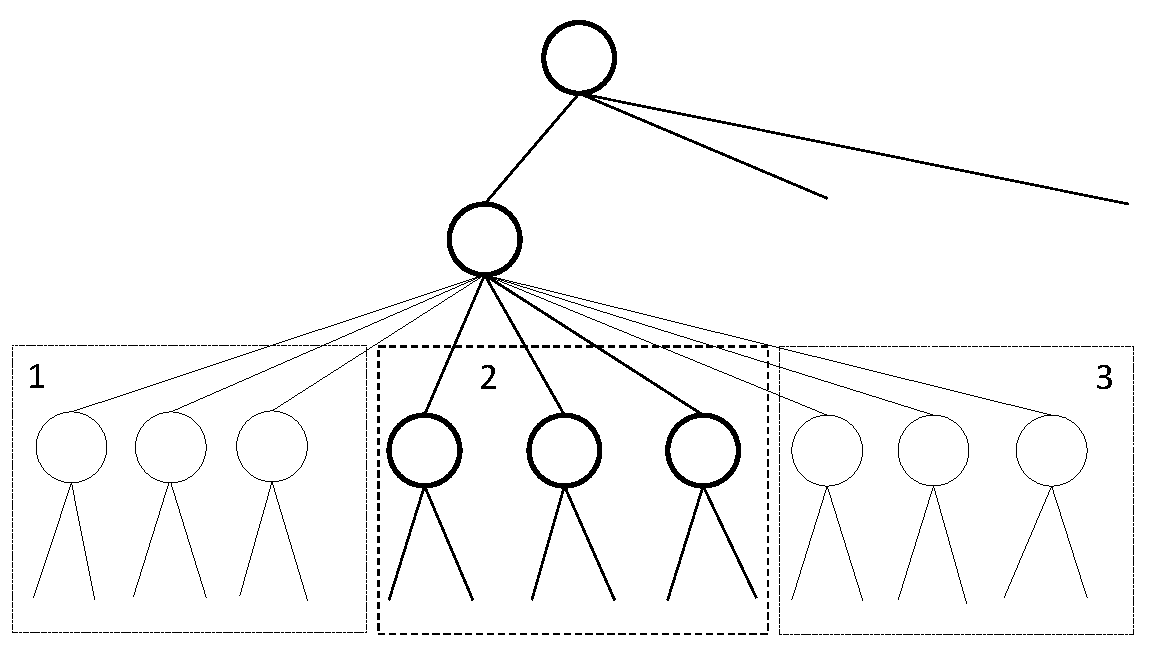
\includegraphics[clip, width=\textwidth]{determinizationc.pdf}
\caption{Example of a determinization with a single tree. In this example, \emph{D} = \{1,2,3\}
and the selected determinization is 2.}
\label{fig:det}
\end{center}
\end{figure}

To deal with games having imperfect information, determinization can be applied in the MCTS engine. The principle behind determinization is that, at the start of each simulation at the root, the hidden information is filled in, while being consistent with the history of the game. 

Determinization has been called ``averaging over clairvoyance'' \cite{russell10},
where players never try to hide or gain information, because in each determinization,
all information is already available. Despite these  shortcomings, it has
produced strong results in the past, for instance in Monte-Carlo engines for the trick-based card game  Bridge \cite{ginsberg99}, the card game Skat \cite{conf/ijcai/BuroLFS09}, Scrabble \cite{sheppard02}, and Phantom Go \cite{cazenave06}. 

Determinization in the MCTS framework has been applied in games such as Scotland Yard \cite{nijssen12tciaig} and Lord of the Rings: The Confrontation \cite{cowling2012}. It works as follows. For each MCTS simulation starting at the root the missing information  is filled in a  random manner. The determinization is used throughout the whole simulation. There are two approaches to build and traverse the search tree. 

The first approach is by generating a separate tree for each determinization \cite{cowling2012}. After selecting a determinization at the root node, the corresponding tree is traversed. Based on majority voting \cite{nijssen12tciaig} the final move can be selected. Each candidate move receives one vote from each tree where it is the move that was played most often. The candidate move with the highest number of votes is selected
as the best move. If more moves are tied, the move with the highest number of visits
over all trees is selected. The concept of separate-tree determinization is similar to root parallelization.

The second approach is using single-tree determinization \cite{ciancarini10,cowling2012,nijssen12tciaig}. When generating the tree, all possible moves from all possible determinizations are generated. When traversing the tree, only the moves consistent with the current determinization are considered. An example is given in \figurename~\ref{fig:det}. The advantage of this technique is that information is shared between different determinizations, increasing the amount of usable information. This type of determinization is  also called Single-Observer Information Set Monte-Carlo Tree Search \cite{cowling2012}.

\section{Sequential Halving and MCTS in Partially Observable Games}
\label{sec:h-mcts}

In this section we describe our approach to applying Hybrid MCTS~\cite{Pepels14hmcts} to partially observable games. Hybrid MCTS is based on the concept of minimizing \emph{simple regret} near the root, and \emph{cumulative regret} in the rest of the tree. Simple regret is defined as the regret of not \emph{recommending} the optimal move. Whereas cumulative regret is the regret over having \emph{selected} suboptimal moves during sampling.

In their analysis of the links between simple and cumulative regret in Multi-Armed Bandits, Bubeck \emph{et al.}~\cite{Bubeck11Pure} found that upper bounds on cumulative regret lead to lower bounds on simple regret, and that the smaller the upper bound on the cumulative regret, the higher the lower bound on simple regret, regardless of the recommendation policy, \ie the smaller the cumulative regret, the larger the simple regret. As such, no policy can give an optimal guarantee on both simple and cumulative regret at the same time. Since UCB gives an optimal upper bound on cumulative regret, it cannot also provide optimal lower bounds on simple regret. Therefore, a combination of different regret minimizing selection methods in the same tree is used in Hybrid MCTS.

This section is structured as follows, first we discuss Sequential Halving, a novel simple regret minimizing algorithm for Multi-Armed Bandits, in Subsection~\ref{subsec:seq_halving}. Next in Subsection~\ref{subsec:h-mcts_po} we discuss how a hybrid search technique may be used in partially observable games.

\subsection{Sequential Halving}
\label{subsec:seq_halving}

\IncMargin{1em}
\begin{algorithm2e}[b]
\setstretch{0.95}
	\KwIn{total budget $T$, $K$ arms}
	\KwOut{recommendation $J_T$}
	\vspace{0.05cm}
	$S_0 \gets \{1,\dots,K\}$,
	$B \gets \ceil{\log_2{K}} - 1$														\;
	\BlankLine
	\For{k=0 \emph{\KwTo} $B$}{
		sample each arm $i \in S_k$, 										
		$n_k = \floor[\bigg]{\frac{T}{|S_k|\ceil{\log_2{|S|}}}}$
		times 																				\;
		\vspace{0.1cm}
		update the average reward of each arm based on the rewards 		\;
		$S_{k+1} \gets$ the $\ceil{|S_k|/2}$ arms from $S_k$ with the best average			\;
	}
	\KwRet{the single element of $S_B$}
  \caption[Sequential Halving]{Sequential Halving~\protect\cite{Karnin13SH}. \label{alg:seqhalv}}
\end{algorithm2e}
\DecMargin{1em}

Non-exploiting selection policies have been proposed to decrease simple regret at high rates in multi-armed bandits. Given that UCB1~\cite{auer2002using} has an optimal rate of cumulative regret convergence, and the conflicting limits on the bounds on the regret types shown in~\cite{Bubeck11Pure}, policies that have a higher rate of exploration than UCB1 are expected to have better bounds on simple regret. Sequential Halving (SH)~\cite{Karnin13SH} is a novel, pure exploration technique developed for minimizing simple regret in the Multi-Armed Bandit (MAB) problem.

In many problems there are only one or two good decisions to be identified, this means that when using a pure exploration technique, a potentially large portion of the allocated budget is spent sampling suboptimal arms. Therefore, an efficient policy is required to ensure that inferior arms are not selected as often as arms with a high reward. Successive Rejects~\cite{audibert2010best} was the first algorithm to show a high rate of decrease in simple regret. It works by dividing the total computational budget into distinct rounds. After each round, the single worst arm is removed from selection, and the algorithm is continued on the reduced subset of arms. Sequential Halving (SH)~\cite{Karnin13SH}, was later introduced as an alternative to Successive Rejects, offering better performance in large-scale MAB problems.

SH divides search time into distinct rounds, and during each round arms are sampled uniformly. After each such round, the empirically worst half of the remaining arms are removed until a single arm remains. The rounds are equally distributed such that each round is allocated approximately the same number of trials (budget), but with smaller subset of available arms to sample. Sequential Halving is detailed in Algorithm~\ref{alg:seqhalv}.

\subsection{Hybrid MCTS for Partially Observable Games}
\label{subsec:h-mcts_po}

In~\cite{Pepels14hmcts} a Hybrid MCTS is proposed. This technique uses recursive Sequential Halving, or SHOT~\cite{Cazenave14SHOT} to minimize simple regret near the root as depicted in Figure~\ref{fig:h-mcts_rounds}. The hybrid technique has shown to improve performance in several domains, including Amazons, AtariGo and Pentalath.  Previous algorithms that use MCTS with simple regret minimizing selection methods showed similar improvements in recommended moves in Markov Decision Processes~\cite{Feldman12BRUE,tolpin2012mcts}.

\begin{figure}[ht]
	\centering
	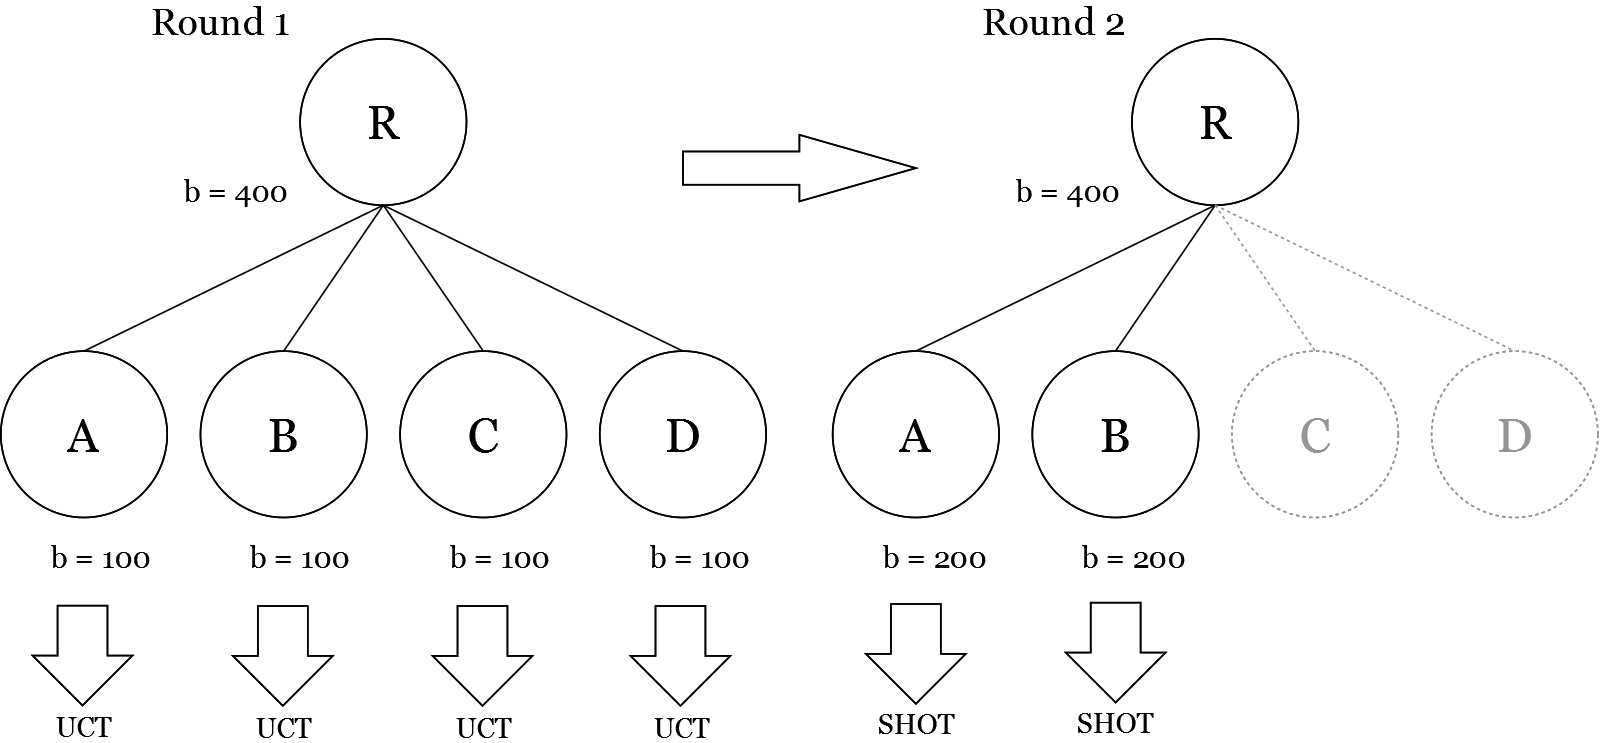
\includegraphics[width=.75\textwidth]{img/H-MCTS_Rounds.png}
	\caption[Hybrid MCTS example rounds]{Example rounds of H-MCTS with a budget limit $B = 150$. Sequential Halving is applied only at the root. On all other plies, UCT in the form of IS-MCTS is applied.}
	\label{fig:h-mcts_rounds}
\end{figure}

In this paper we extend Hybrid MCTS to partially observable games. The problem with these domains is that when using multiple determinizations during search, revisiting nodes may result in different playable moves. This is not a problem when using selection methods such as UCT, which are greedy and select moves based on the current statistics. However, because SH is a uniform exploration method, in order to guarantee its lower bound on simple regret must be able to revisit the same node multiple times. In other words, available moves should not change in between visits of the algorithm, or its specifically designed budget allocation is no longer valid.

In all partially observable games, the current player always has knowledge over the current set of moves that he can play. Therefore, at the root of the search tree, moves are consistent between visits. As such, SH can be used to uniformly explore moves at the root without problems. 

The approach is detailed in Algorithm~\ref{alg:seqhalv-mcts}. At the root, budget is allocated according to SH. For each sample, the appropriate IS-MCTS implementation can be used~\cite{cowling2012}. For this paper, based on our experimental domains (Section~\ref{sec:exp_dom}, we use single observer IS-MCTS.

\IncMargin{1em}
\begin{algorithm2e}[ht]
\setstretch{0.95}
	\KwIn{total budget $T$, $K$ moves}
	\KwOut{recommendation $J_T$}
	\vspace{0.05cm}
	$S_0 \gets \{1,\dots,K\}$,
	$B \gets \ceil{\log_2{K}} - 1$														\;
	\BlankLine
	\For{k=0 \emph{\KwTo} $B$}{
		\For{each move $i \in S_k$} {									
		  $n_k \gets \floor[\bigg]{\frac{T}{|S_k|\ceil{\log_2{|S|}}}}$ \;
		  \For{n=0 \emph{\KwTo} $n_k$} {
		  	select a new determinization $d$ at random 							\; \label{determinize}
		 	sample move $i$ using {\sc IS-MCTS} and determinization $d$ 				\;
		 	update the average of $i$ reward based on the sample 		\;
		  }
		}
		\vspace{0.1cm}
		$S_{k+1} \gets$ the $\ceil{|S_k|/2}$ moves from $S_k$ with the best average			\;
	}
	\KwRet{the single element of $S_B$}
  \caption[Sequential Halving]{Sequential Halving and Information Set MCTS~\protect. \label{alg:seqhalv-mcts}}
\end{algorithm2e}
\DecMargin{1em}

\section{Experimental Domains}
\label{sec:exp_dom}

In this section we discuss the partially observable games which are used in the experiments in Section \ref{sec:exp_res}. First we describe the two stochastic domains Go Fish and Lost Cities. Next the deterministic games Phantom Domineering and Phantom Go are explained.

\subsection{Stochastic Games}

We describe two stochastic domains. In both games, cards are drawn from a randomly shuffled deck, limiting the possible predictions of future states. Moreover, in both games, moves available to the opponent are either partially or completely invisible. However, whenever a move is made, it becomes immediately known to both players. As these games progress, more information regarding the actual game state becomes available to both players.

{\sc \bf Go Fish} is a card game which is generally played by multiple players. The goal is to collect as many `books' of 4 cards of equal rank. All players hide their cards from each other, and only finished books of four cards are placed face-up on the table. Each turn, a player may ask a single other player for a specific rank. If the questioned player has any cards of the requested rank in his hand, he gives them to the requesting player, which may consequently make a new request. If the questioned player does not posses a card of the requested rank, the questioning player must `go fish', drawing a card from the stack, and the turn moves to the next player. The game ends when there are no more cards on the stack, and the player with the most finished books wins the game.

In our implementation, the game was slightly modified to allow it to be played by two players. Both players receive seven cards in hand at the start of the game. Moreover, the finished books are not similarly rewarded. Books of numbered cards give a score of one, whereas books of face cards assign a score of two, a book of aces gives a score of three. As a result, when the game ends, the player with the highest score wins.

The game state is determinized by removing the from the non-visible player's all card drawn from the deck, shuffling the deck and re-drawing the non-visible player's hand. This means that whenever a card was obtained from the opponent it is no longer treated as invisible, because it cannot be anywhere else than in the opponent's hand or visible on the table in a finished book.

{\sc \bf Lost Cities} is a card game, designed in 1999 by Reiner Knizia. The goal of the game is to achieve the most profitable set of expeditions to one or more of five lost cities. Players start expeditions by placing numbered cards on them, each player can start up to five expeditions regardless of the opponents' expeditions. Each card in the game has a color and a number, the colors represent one of the five expeditions, the numbers representing the score gained. Next to these cards, colored investment cards cumulatively double the score awarded for an expedition. The deck consists of 60 cards, nine numbered cards per color, and three investment cards per color.

Placing a card on an empty expedition `initializes' it with a cost of 20. Or, when an investment card is played, with a score of $20\times I_c$, where $I_c$ is the number of investment cards played on expedition $c$. These cards can only be played on an expedition when no other cards have been played on it. For example, playing the `red 5' card starts the red expedition with a cost of 20 and a score of 5 resulting in a -15 score for the player. With a single investment card on this expedition, the score will be 30. Playing more cards on the expedition leads to higher scores. However, only increasing cards may be placed on top of others. In this example, the card `red 3' can no longer be played, whereas the `red 8' card can be played.

Each turn, players may either play or discard a card, and draw a card from the draw pile or one of the discard piles. Discarding a card places it on top of one of the colored discard piles which are accessible to both players. The game ends when no cards are left on the draw pile, the player with the highest score wins the game.

In Lost Cities, interaction between players is limited. However, players have to carefully chose their expeditions partly based on their opponents choices. Moreover, players must be careful not to discard cards which may benefit their opponent, but at the same time take care that they can draw cards beneficial to their chosen expeditions. 

As in Go Fish, the game state is determinized by removing the non-visible player's hand, shuffling the deck and re-drawing the non-visible player's hand.

\subsection{Deterministic Games}

We describe two so-called phantom games. Phantom games are modified versions of fully observable games, in which part of the game state is made invisible to the players. Both games are otherwise fully deterministic, \ie no roll of the dice, or drawing cards. Consequently, whenever a player makes a move it may be rejected, the player may move again until his move is no longer rejected. Playing a move that is rejected is always beneficial, since it provides the player with new information of the actual game state.

{\sc \bf Phantom Domineering} is based on the combinatorial game Domineering, which is generally played on a square board with two players. Each turn players block two adjacent positions on the board, one player plays vertically, and the other horizontally. The game ends when one of the players cannot make move. As with most combinatorial games, the first player unable to make a move loses the game, and draws are not possible.

In Phantom Domineering, players can only directly observe their own pieces on the board. For both players, their opponent's pieces are hidden, and can only be observed indirectly by performing rejected moves. A unique property in Phantom Domineering is that rejected moves do not provide immediate information about the opponent's moves. In games where moves consist of occupying single positions, a rejected move can immediately reveal an opponent's move. In Phantom Domineering, however, a rejected move means that either one of the two positions is blocked, or both. Therefore, when determinizing, all opponent's stones are first replaced such that they match the rejected moves, after this, all remaining stones are placed randomly on the board.

{\sc \bf Phantom Go} is version of Go played in which the opponent's are not revealed. When a move is illegal it is usually because there is an opponent's stone on the chosen intersection. In this case a referee publicly announces that the player made an illegal move and the same player may move again. The Chinese rules are used for scoring games. During the determinization opponent stones are placed on previous illegal moves. The remaining opponent stones are place randomly on the determinized board~\cite{cazenave06}. The principle of our engine: {\sc GoLois}, is to perform one play-out per determinization. For each possible move, a great number of determinizations followed by a play-out are performed. The move with the highest average is then chosen. Using this approach, {\sc GoLois} won the gold medal in 5 of the 6 Phantom Go tournaments held during the last Computer Olympiads. Phantom Go is played by humans at Go congresses and is enjoyed by spectators who can see both players' boards as well as the complete referee board.

\section{Experiments and Results}
\label{sec:exp_res}
In this section we show the results of the experiments performed on four, partially observable two-player games. H-MCTS and the games were implemented in two different engines. Go Fish, Lost Cities and Phantom Domineering are implemented in a Java based engine. Phantom Go is implemented in the \emph{C++} based engine {\sc GoLois}.

Lost Cities relies heavily on a heuristic play-out function which prevents obvious bad moves such as starting an expedition without a chance of making a profit. These heuristics improve play over a random play-out by up to $40\%$. In Phantom Domineering, an $\epsilon$-greedy play-out strategy selects moves based on the number of available moves for the opponent $n_o$ and the player to move $n_p$ and selects the move which maximizes $n_p - n_o$. For both Go Fish and Phantom Go, moves are selected uniformly random during play-outs.

In the next subsection, we run experiments on our experimental domains using a set of different algorithms:
\begin{itemize}
\item \textbf{H-MCTS} selects moves according to Sequential Halving at the root and UCT in all other parts of the tree, according to Algorithm~\ref{alg:seqhalv-mcts}. In all domains, single observer IS-MCTS~\cite{cowling2012} is used.
\item \textbf{SH} selects among available moves according to Sequential Halving (Algorithm~\ref{alg:seqhalv}), and samples the moves by play-out immediately. As such, no search is performed.
\item \textbf{MCTS} selects moves using UCT from root to leaf. As in {\sc H-MCTS}, single observer IS-MCTS is used.
\item \textbf{UCB} selects among available moves according to the UCT selection method (Equation~\ref{eq:uct}) and samples the move immediately by play-out. As such, no search is performed. The method is similar to using the UCB1 algorithm for MABs.
\end{itemize}
In all experiments, and for all algorithms, a new determinization is uniformly selected for each simulation. For each individual game, the $C$ constant, used by UCT (Equation \ref{eq:uct}) was tuned. MCTS, UCB and H-MCTS use the same value for the $C$ constant in all experiments.

\subsection{Results}
\label{subsec:results}

For each table, the results are shown with respect to the row algorithm, along with a 95\% confidence interval. For each experiment, the players' seats were swapped such that 50\% of the games are played as the first player, and 50\% as the second, to ensure no first-player or second-player bias. Because H-MCTS cannot be terminated any-time we present only results for a fixed number of simulations. In each experiment, both players are allocated a budget of either 10,000, or 25,000 play-outs. In all tables, significantly positive results are bold-faced.

\begin{table}[ht]
\centering
\setlength{\tabcolsep}{10pt}

\begin{tabular}{@{}lrrrr@{}}
\toprule
& \multicolumn{4}{c}{\textbf{Go Fish}} \\
& \multicolumn{1}{c}{\textbf{H-MCTS}} & \multicolumn{1}{c}{\textbf{SH}} & \multicolumn{1}{c}{\textbf{MCTS}} & \multicolumn{1}{c}{\textbf{UCB}} \\[1mm] \cmidrule(l){2-5} 
\textbf{H-MCTS} & \multicolumn{1}{c}{-}		& \textbf{60.9\%}$\pm$2.9 	& \textbf{54.3\%}$\pm$1.9 	& \textbf{62.3\%}$\pm$2.9 	\\[.5mm] 
\textbf{SH}     & 39.1\%$\pm$2.9 			& \multicolumn{1}{c}{-} 	& 44.0\%$\pm$3.0 			& 51.3\%$\pm$2.0 			\\[.5mm] 
\textbf{MCTS}   & 45.7\%$\pm$1.9 			& \textbf{56.0\%}$\pm$3.0 	& \multicolumn{1}{c}{-} 	& \textbf{55.0\%}$\pm$3.1 	\\[.5mm]
\textbf{UCB}	& 37.7\%$\pm$2.9			& 48.7\%$\pm$2.0 			& 45.0\%$\pm$3.1 			& \multicolumn{1}{c}{-} 	\\[.5mm] 
\end{tabular}

\begin{tabular}{@{}lrrrr@{}}
\toprule
& \multicolumn{4}{c}{\textbf{Lost Cities}} \\
& \multicolumn{1}{c}{\textbf{H-MCTS}} & \multicolumn{1}{c}{\textbf{SH}} & \multicolumn{1}{c}{\textbf{MCTS}} & \multicolumn{1}{c}{\textbf{UCB}} \\ [1mm] \cmidrule(l){2-5} 
\textbf{H-MCTS} & \multicolumn{1}{c}{-}		& 46.1\%$\pm$3.1 			& \textbf{54.1\%}$\pm$3.1  	& 47.1\%$\pm$3.1 			\\[.5mm] 
\textbf{SH}     & \textbf{53.9\%}$\pm$3.1 	& \multicolumn{1}{c}{-} 	& \textbf{55.6\%}$\pm$1.9  	& 50.1\%$\pm$1.9  			\\[.5mm] 
\textbf{MCTS}   & 45.9\%$\pm$3.1		 	& 44.4\%$\pm$1.9  			& \multicolumn{1}{c}{-} 	& 45.3\%$\pm$3.1  			\\[.5mm]
\textbf{UCB}	& 52.9\%$\pm$3.1			& 49.9\%$\pm$1.9  			& \textbf{54.7\%}$\pm$3.1 	& \multicolumn{1}{c}{-} 	\\[.5mm]
\end{tabular}

\begin{tabular}{@{}lrrrr@{}}
\toprule
& \multicolumn{4}{c}{\textbf{8$\times$8 Phantom Domineering}}       \\
& \multicolumn{1}{c}{\textbf{H-MCTS}} & \multicolumn{1}{c}{\textbf{SH}} & \multicolumn{1}{c}{\textbf{MCTS}} & \multicolumn{1}{c}{\textbf{UCB}} \\ [1mm] \cmidrule(l){2-5} 
\textbf{H-MCTS} & \multicolumn{1}{c}{-}		& 45.1\%$\pm$3.1			& \textbf{59.9\%}$\pm$3.0 	& \textbf{59.5\%}$\pm$3.0 		\\[.5mm] 
\textbf{SH}     & \textbf{54.9\%}$\pm$3.1	& \multicolumn{1}{c}{-}		& \textbf{55.1\%}$\pm$3.1	& \textbf{58.6\%}$\pm$3.1 		\\[.5mm] 
\textbf{MCTS}   & 41.1\%$\pm$3.0			& 44.9\%$\pm$3.1			& \multicolumn{1}{c}{-} 	& 49.4\%$\pm$3.1  				\\[.5mm] 
\textbf{UCB}	& 40.5\%$\pm$3.0			& 41.4\%$\pm$3.1			& 51.6\%$\pm$3.1			& \multicolumn{1}{c}{-} 		\\[.5mm] \bottomrule
\end{tabular}

\vspace{2mm}
{\caption{Win rates with respect to the row player. Minimum of 1,000 games per experiment, 10,000 simulations per move.} \label{tab:results_10k}}
\end{table}

\begin{table}[ht]
\centering
\setlength{\tabcolsep}{10pt}

\begin{tabular}{@{}lrrrr@{}}
\toprule
& \multicolumn{4}{c}{\textbf{Go Fish}} \\
& \multicolumn{1}{c}{\textbf{H-MCTS}} & \multicolumn{1}{c}{\textbf{SH}} & \multicolumn{1}{c}{\textbf{MCTS}} & \multicolumn{1}{c}{\textbf{UCB}} \\[1mm] \cmidrule(l){2-5} 
\textbf{H-MCTS} & \multicolumn{1}{c}{-}		& \textbf{62.2\%}$\pm$2.9 	& \textbf{55.2\%}$\pm$3.0 	& \textbf{61.8\%}$\pm$2.9 	\\[.5mm] 
\textbf{SH}     & 42.2\%$\pm$3.0 			& \multicolumn{1}{c}{-} 	& 42.2\%$\pm$3.0 			& 51.7\%$\pm$3.1 			\\[.5mm] 
\textbf{MCTS}   & 44.9\%$\pm$3.0			& \textbf{57.9\%}$\pm$3.0 	& \multicolumn{1}{c}{-} 	& \textbf{59.0\%}$\pm$3.0 	\\[.5mm]
\textbf{UCB}	& 38.2\%$\pm$2.9			& 48.3\%$\pm$3.1			& 41.0\%$\pm$3.1 			& \multicolumn{1}{c}{-} 	\\[.5mm] 
\end{tabular}

\begin{tabular}{@{}lrrrr@{}}
\toprule
& \multicolumn{4}{c}{\textbf{Lost Cities}} \\
& \multicolumn{1}{c}{\textbf{H-MCTS}} & \multicolumn{1}{c}{\textbf{SH}} & \multicolumn{1}{c}{\textbf{MCTS}} & \multicolumn{1}{c}{\textbf{UCB}} \\ [1mm] \cmidrule(l){2-5} 
\textbf{H-MCTS} & \multicolumn{1}{c}{-}		& 48.6\%$\pm$1.9 			& \textbf{52.7\%}$\pm$1.9		  	& 44.9\%$\pm$3.0 	\\[.5mm] 
\textbf{SH}     & 51.4\%$\pm$1.9 			& \multicolumn{1}{c}{-} 	& \textbf{57.6\%}$\pm$3.1  	& 52.8\%$\pm$3.1  			\\[.5mm] 
\textbf{MCTS}   & 47.4\%$\pm$1.9		 	& 42.4\%$\pm$3.0  			& \multicolumn{1}{c}{-} 	& 43.7\%$\pm$1.9  			\\[.5mm]
\textbf{UCB}	& \textbf{55.1\%}$\pm$3.1	& 47.3\%$\pm$3.1  			& \textbf{56.3\%}$\pm$1.9 	& \multicolumn{1}{c}{-} 	\\[.5mm]
\end{tabular}

\begin{tabular}{@{}lrrrr@{}}
\toprule
& \multicolumn{4}{c}{\textbf{8$\times$8 Phantom Domineering}}       \\
& \multicolumn{1}{c}{\textbf{H-MCTS}} & \multicolumn{1}{c}{\textbf{SH}} & \multicolumn{1}{c}{\textbf{MCTS}} & \multicolumn{1}{c}{\textbf{UCB}} \\ [1mm] \cmidrule(l){2-5} 
\textbf{H-MCTS} & \multicolumn{1}{c}{-}		& 48.9\%$\pm$3.1			& 53.0\%$\pm$3.1 			& \textbf{54.5\%}$\pm$3.1 		\\[.5mm] 
\textbf{SH}     & 51.1\%$\pm$3.1			& \multicolumn{1}{c}{-}		& \textbf{56.1\%}$\pm$3.1	& 51.8\%$\pm$3.1		 		\\[.5mm] 
\textbf{MCTS}   & 47.0\%$\pm$3.1			& 43.9\%$\pm$3.1			& \multicolumn{1}{c}{-} 	& 51.3\%$\pm$3.1  				\\[.5mm] 
\textbf{UCB}	& 45.6\%$\pm$3.1			& 48.7\%$\pm$3.1			& 51.3\%$\pm$3.1			& \multicolumn{1}{c}{-} 		\\[.5mm] \bottomrule
\end{tabular}

\vspace{2mm}
{\caption{Win rates with respect to the row player. Minimum of 1,000 games per experiment, 25,000 simulations per move.} \label{tab:results_25k}}
\end{table}

Tables~\ref{tab:results_10k} and~\ref{tab:results_25k} show the comparative results for search performed with 10,000 and 25,000 simulations per move, respectively. First, results show that only in Go Fish did performing search improve performance over flat Monte-Carlo sampling, in both Lost Cities and Phantom Domineering performing search did not improve performance. This coincides with previous results for Phantom Go, for which it was determined that search could did not perform better than UCB sampling. 

In all games, using H-MCTS improves performance over MCTS when sampling 10,000 simulations per move. In the 25,000 case, MCTS and UCB's performances appear to recover in Lost Cities and Phantom Go. In Go Fish, performance is stable with respect to the number of simulations. For the games where performing search does not improve performance over single-ply sampling, SH is either on par or outperforms UCB.

In all cases, in both experimental setups, SH or H-MCTS either outperforms MCTS and UCB significantly, or does not negatively impact performance. In Phantom Domineering, sampling using SH improves performance over UCB by up to 8.6\%. A significant improvement when considering that no knowledge or heuristics were introduced in the search. Moreover, SH improves the performance of the award-winning engine {\sc GoLois} by up to 7.1\% over UCB, as shown in Table~\ref{tab:ph_go}. In this table we detail the results over different $C$ constants for UCB, showing that without tuning any parameter, SH is able to outperform UCB in all cases. UCB's performance similarly somewhat recovers when given more simulations. However, in all but one case (when $C=0.4$), SH still significantly outperforms UCB with 25,000 simulations per move.

\begin{table}[ht]
\centering
\setlength{\tabcolsep}{10pt}
\begin{tabular}{@{}llrr@{}}
\toprule
& & \multicolumn{2}{c}{\textbf{Phantom Go}} \\
& & \multicolumn{1}{c}{10,000} & \multicolumn{1}{c}{25,000} \\
& \multicolumn{1}{c}{$C$} & \multicolumn{1}{c}{Simulations} & \multicolumn{1}{c}{Simulations} \\ [1mm] \cmidrule(l){1-4}
\textbf{SH} vs. \textbf{UCB}  & 0.1 & \textbf{69.6\%}$\pm$2.9 & \textbf{70.6\%}$\pm$2.9 \\ [.5mm]
 & 0.2 & \textbf{58.8\%}$\pm$3.1 & \textbf{58.6\%}$\pm$3.1 \\[.5mm]
 & 0.3 & \textbf{58.1\%}$\pm$3.1 & \textbf{54.3\%}$\pm$3.1 \\[.5mm]
 & 0.4 & \textbf{58.0\%}$\pm$3.1 & 53.0\%$\pm$3.1          \\[.5mm]
 & 0.5 & \textbf{57.1\%}$\pm$3.1 & \textbf{55.3\%}$\pm$3.1 \\[.5mm]
 & 0.6 & \textbf{59.1\%}$\pm$3.1 & \textbf{51.9\%}$\pm$3.1 \\[.5mm]
 & 0.7 & \textbf{60.3\%}$\pm$3.1 & \textbf{56.7\%}$\pm$3.1 \\[.5mm]
 & 0.8 & \textbf{61.5\%}$\pm$3.1 & \textbf{58.6\%}$\pm$3.1 \\[.5mm]
 & 0.9 & \textbf{64.5\%}$\pm$3.0 & \textbf{57.8\%}$\pm$3.1 \\[.5mm]
\bottomrule
\end{tabular}
\vspace{2mm}
{\caption{Experimental results for Phantom Go. SH vs. UCB with varying $C$ constant. 1,000 games, win rates with respect to SH.} \label{tab:ph_go}}
\end{table}

\section{Conclusions}
\label{sec:concl}

\bibliographystyle{splncs03}
\bibliography{h-mcts}
\end{document}
